\documentclass[landscape,footrule]{foils}
\usepackage[lecture-serie]{foiltex-extra}
\usepackage{crysymb}
\usepackage{graphics}
\usepackage[pdftex]{graphicx} 




\newcommand{\lecture}{Model-based Clustering}
\newcommand{\lserie}{LTAT.02.004 Machine Learning II}
\newcommand{\ldate}{April 23, 2019}
\newcommand{\lauthor}{Sven Laur}
\newcommand{\linst}{University of Tartu}
\graphicspath{{./illustrations/}}
%\MyLogo{\lserie,\  ML and MAP estimates, \ldate}


\newcommand{\leqm}{\ \leq_m}


\newcommand{\bigvskip}{\vskip 2em}
\newcommand{\lastline}{\vspace*{-2ex}}
\newcommand{\spreadappart}{\vspace*{\fill}}


\newcommand{\pd}[1]{\mathrm{p}[#1]}

\begin{document}
\titlefoil



\foilhead[-1cm]{Ancestral reconstruction}

\textbf{General formulation.}
Given a set of objects that are created by noisy reproduction procedure find out which of them is a true original.

\begin{diamonds}
\item Find out how species have been evolving using DNA samples
\item Find out which of the ancient manuscripts is the original
\item Find out the source of a gossip and evaluation of internet memes
\item Find out how academic texts are plagiarised  
\end{diamonds}
\vspace*{2cm}

\textbf{General principle.} Errors made by the coping mechanism are very likely to be propagated to the further copies.
\begin{triangles}
\item The copy without errors (\emph{mutations}) must be the true original.
\item To reconstruct evolutionary tree we must back-track all mutations.
\end{triangles}

\foilhead[-1cm]{Illustrative example}

Assume that we know the true original and there are four possible errors in documents. Then we can construct error vectors and define a set of plausible evolutionary explanations. One of them is depicted below.\vspace*{1cm}


\illustration[scale=0.9]{complex-mutation-tree}
\vspace*{0.5cm}

In most cases the copying procedure is almost perfect and occurrence of a single error is much more likely than the occurrence of two or more errors.\vspace*{-0.5cm}   

\foilhead[-1cm]{Illustrative example continued}

The evolutionary tree presented in the previous slide contains six mutations, whereas more plausible explanation below contains only four mutations.\vspace*{1cm}

\illustration[scale=0.9]{simple-mutation-tree}
\vspace*{0.5cm}

\foilhead[-1cm]{Naive mutation model}

\begin{triangles}
\item All sites are independently flipped with probability $p$
\item A child is obtained form a parent through a single copying operation
\item A copying operations are independent form each other
\end{triangles}
\vspace*{1cm}


\textbf{Correponding mathematical model.}
Let $h(\vec{u},\vec{v})=\#\set{i: u_i\neq v_i}$ and $n$ the length of vectors. Then  the probability that $\vec{v}$ is child of $\vec{u}$ is
\begin{align*}
\pr{\vec{u}\to\vec{v}}=(1-p)^{n-h(\vec{u},\vec{v})}p^{h(\vec{u},\vec{v})}
\end{align*}
The probability of the entire tree is the product of edge probabilities:
\begin{align*}
\pr{\TTT}=\prod_{\vec{u}\to\vec{v}}\pr{\vec{u}\to\vec{v}}= \prod_{\vec{u}\to\vec{v}}(1-p)^{n}\left(\frac{p}{1-p}\right)^{h(\vec{u},\vec{v})}
\end{align*}

\foilhead[-1cm]{Corresponding minimisation task}

Let $E$ denote the set of edges in the evolutionary tree. Then we can express 
\begin{align*}
\log \pr{\TTT}=\abs{E}\cdot n\cdot\log(1-p)+\log\left(\frac{p}{1-p}\right)\cdot \sum_{\vec{u}\to\vec{v}} h(\vec{u},\vec{v})
\end{align*}
By dividing log-likelihood with a constant $n\cdot\log(1-p)$ we get a simpler minimisation goal:
\begin{align*}
\abs{E}+\tau(p)\cdot \sum_{\vec{u}\to\vec{v}} h(\vec{u},\vec{v})\to\min
\end{align*}
which implies that for trees with equal size we should take the one with fewer changes. For different tree sizes, the choice depends on $\tau(p)$ value. 


\foilhead[-1cm]{Internet meme evolution}
\enlargethispage{1cm}

\textbf{General setup.} Meme generation is done in modification phases:
\begin{triangles}
\item First, the seed meme $\vec{x}_0$ is generated.
\item Next $\vec{x}_{i+1}$ is generated from $\vec{x}_j$ by altering it.
\item Finally, the phase is ended by choosing a new seed meme. \vspace*{2ex}
\end{triangles} 


\textbf{Modification mechanism}
\begin{triangles}
\item We choose $j$ uniformly from set $\set{0, \ldots, i}$.\vspace*{2ex} 
\end{triangles}

\textbf{Termination of a modification phase}
\begin{triangles}
\item At each time-step we choose a new seed with probability $\varrho$.\vspace*{2ex} 
\end{triangles}

\textbf{Seed generation mechanism}
\begin{triangles}
\item We generate new seed by altering a random $\vec{x}_j$ from the last phase.\vspace*{1ex} 
\end{triangles}


\foilhead[-1cm]{Simplified example. Nearest linkage}

\centerline{
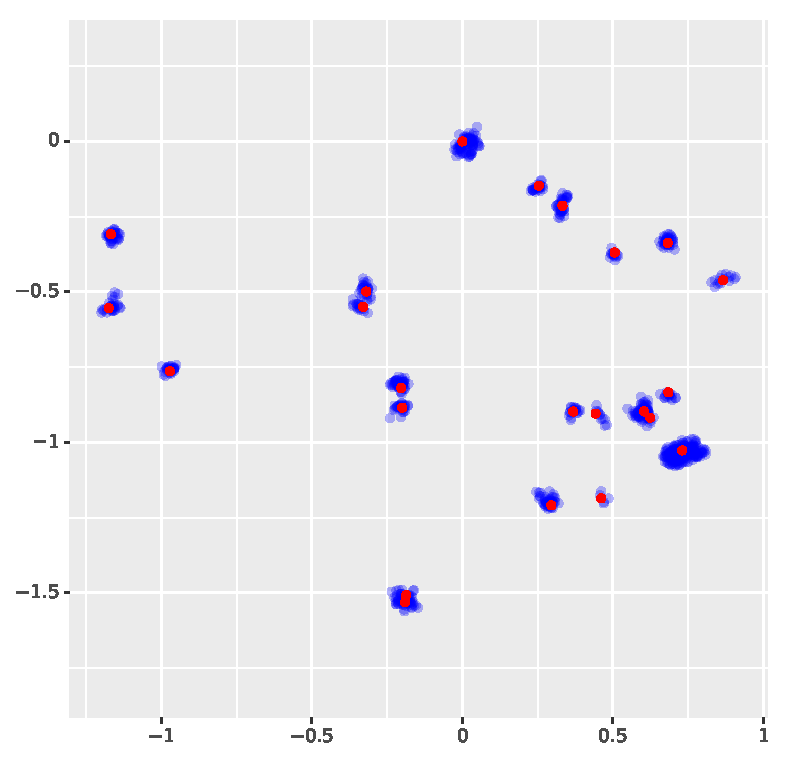
\includegraphics[scale=0.55]{meme_generation_i}
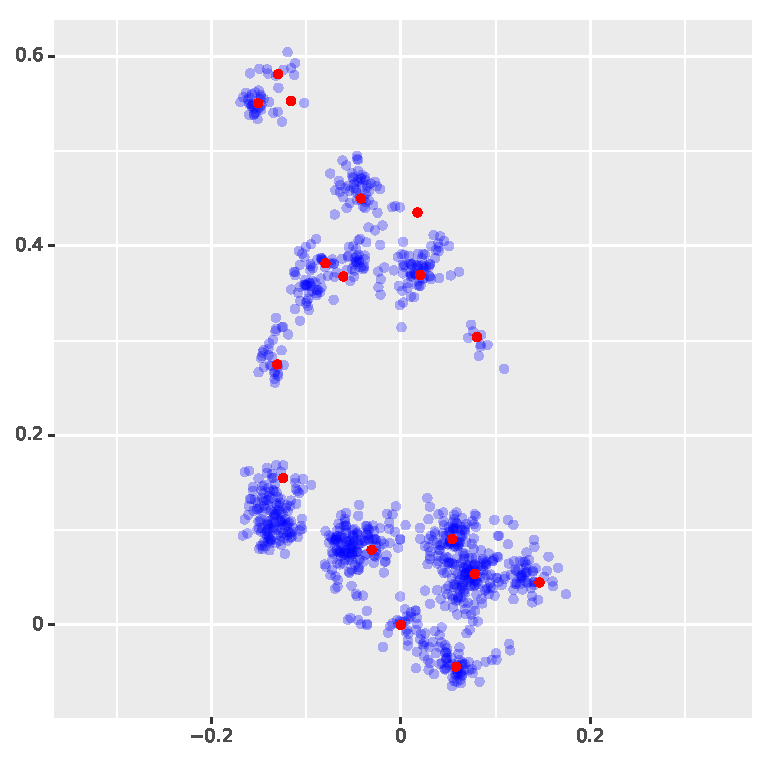
\includegraphics[scale=0.55]{meme_generation_ii}
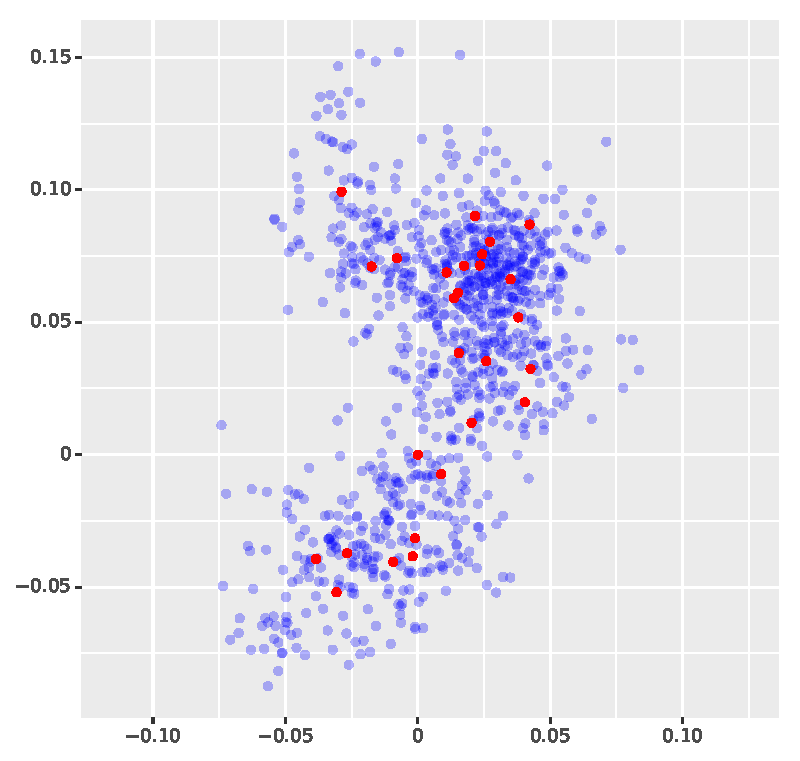
\includegraphics[scale=0.55]{meme_generation_iv}}

\begin{triangles}
\item We do know how many seeds are generated.
\item We do not know the which observations belong to which phases.
\item The closest neighbour of a point is most probably modification.
\item By linking closest points together we can restore a cluster.
\item At some point we start to merge clusters but hopefully we see it.
\end{triangles}


\foilhead[-1cm]{Fast meme generation}

\textbf{General setup.} Meme generation is done in modification phases:
\begin{triangles}
\item First, the seed meme $\vec{x}_0$ is generated.
\item Next $\vec{x}_{i+1}$ is generated from the seed $\vec{x}_0$ by altering it.
\item Finally, the phase is ended by choosing a new seed meme. \vspace*{2ex}
\end{triangles} 


\textbf{Modification mechanism}
\begin{triangles}
\item The choice of alteration mechanism is application specific.\vspace*{2ex} 
\end{triangles}

\textbf{Termination of a modification phase}
\begin{triangles}
\item At each time-step we choose a new seed with probability $\varrho$.\vspace*{2ex} 
\end{triangles}

\textbf{Seed generation mechanism}
\begin{triangles}
\item We generate new seed by altering a seed $\vec{x}_0$ from the last phase.\vspace*{1ex} 
\end{triangles}

\foilhead[-1cm]{Simplified example. Centroid linkage}

\centerline{
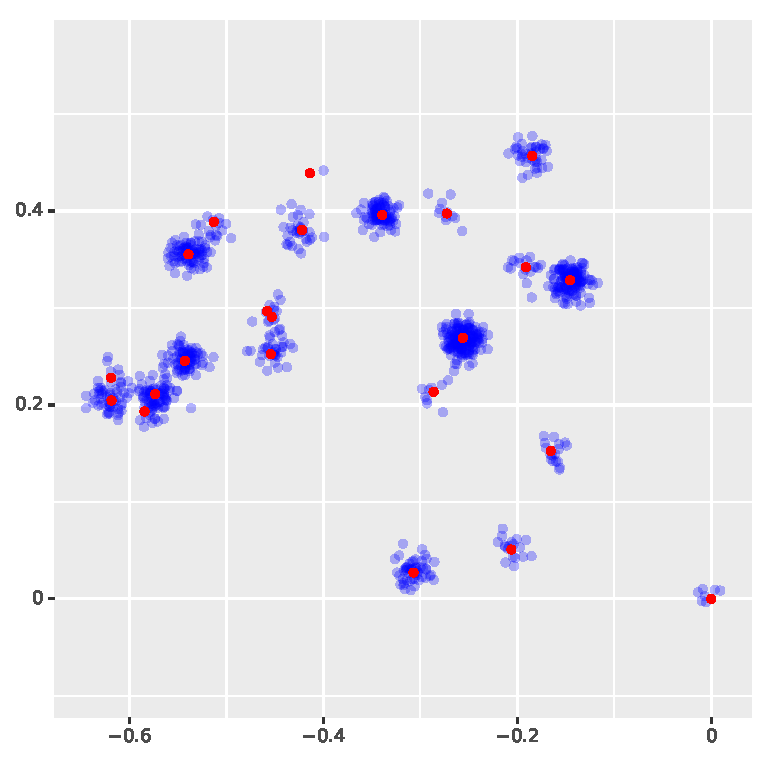
\includegraphics[scale=0.55]{fast_meme_generation_ii}
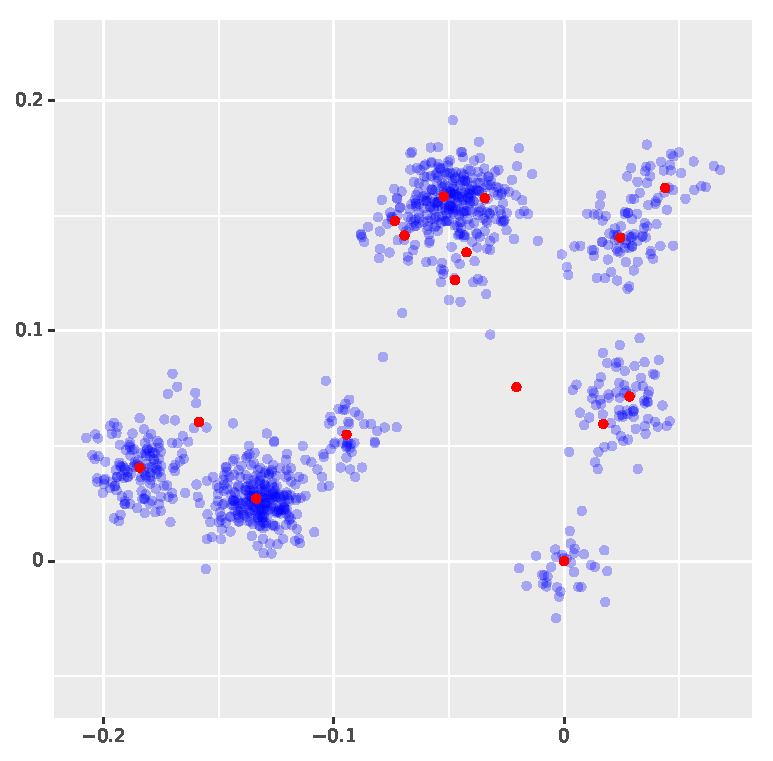
\includegraphics[scale=0.55]{fast_meme_generation_iii}
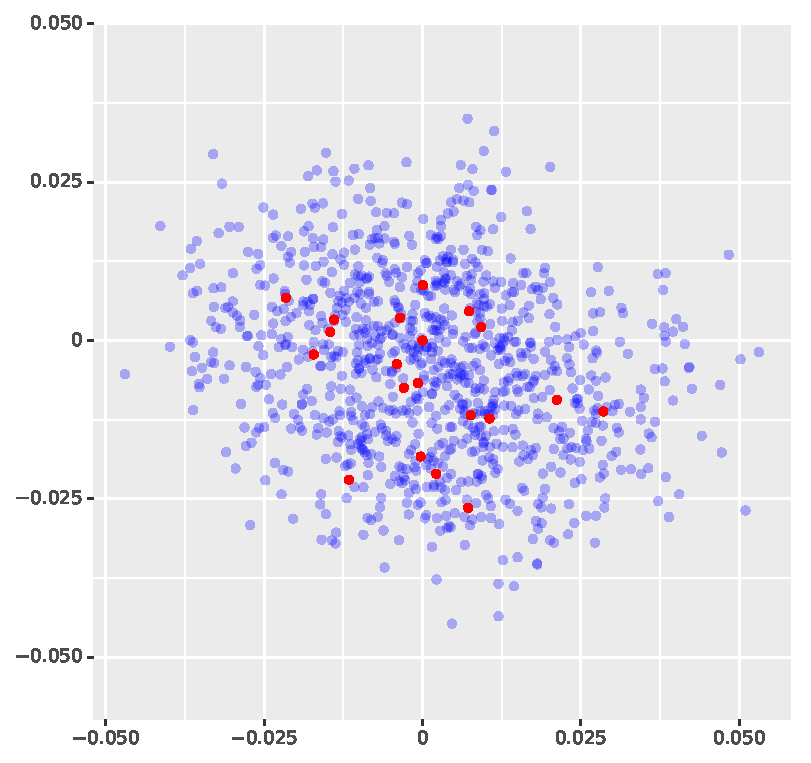
\includegraphics[scale=0.55]{fast_meme_generation_iv}}

\begin{triangles}
\item We do know how many seeds are generated.
\item We do not know the which observations belong to which phases.
\item The closest neighbour of a point is most probably in the same cluster.
\item Centres for connected points are an estimate of a seed.
\item At some point we start to merge clusters but hopefully we see it.
\end{triangles}



\foilhead[-0cm]{Target reconstruction in shooting}

\illustration[scale=0.9, trim = 5cm 2.5cm 5cm 2cm, clip]{shooting-target}

Find the true target for each shooter given that errors in all directions are equiprobable and distributed according to normal distribution.\vspace*{-1cm}

\foilhead[-0cm]{Target reconstruction in shooting}

\illustration[scale=0.9, trim = 5cm 2.5cm 5cm 2cm, clip]{shooting-target-precise}

Reconstruction of the true targets is straightforward when we know the origin of individual shots. We discuss later how to do it exactly.\vspace*{-1cm}

\foilhead[-0cm]{Target reconstruction in shooting}

\illustration[scale=0.9, trim = 5cm 2.5cm 5cm 2cm, clip]{shooting-target-blinded}

Reconstruction of the true targets is much harder if we have to guess the origin of shots by ourselves. This task is known as clustering.\vspace*{-1cm}


\foilhead[-1cm]{Naive probabilistic model}

\begin{triangles}
\item There are $k$ different data sources $\DDD_1,\ldots,\DDD_k$
\item Each data source has a fixed centre $\vec{\mu}_j\in\RR^d$
\item For each data point noise $\varepsilon_t\gets\NNN(0,\sigma)$ for each coordinate
\item To sample data from the distribution $\DDD_j$, we output $\vec{x}=\vec{\mu}_j+\vec{\varepsilon}$ 
\end{triangles}
\vspace*{1cm}

\textbf{Correponding mathematical model.} Let $z_1,\ldots, z_n$ denote assigned labels and $\vec{x}_1,\ldots,\vec{x}_n$ locations of individual data points. Then
\begin{align*}
\pd{\vec{x}_i|z_i=j,\vec{\mu}_j,\sigma}&=\prod_{t=1}^d\frac{1}{\sqrt{2\pi}\sigma}\cdot\exp{-\frac{(x_{it}-\mu_{jt})^2}{2\sigma^2}}\\
\pd{\vec{x}_1,\ldots,\vec{x}_n|\vec{z},\vec{\mu}_1,\ldots,\vec{\mu}_k,\sigma}&=\prod_{i=1}^n
\prod_{t=1}^d\frac{1}{\sqrt{2\pi}\sigma}\cdot\exp{-\frac{(x_{it}-\mu_{z_it})^2}{2\sigma^2}}
\end{align*}


\foilhead[-1cm]{Corresponding minimisation task}
\enlargethispage{1cm}
Again it makes sense to maximise log-likelihood instead of likelihood
\begin{align*}
\log \pd{\vec{x}_1,\ldots,\vec{x}_n|\vec{z},\vec{\mu}_1,\ldots,\vec{\mu}_1,\sigma}&= C(\sigma) - 
\sum_{i=1}^n
\sum_{t=1}^d\frac{(x_{it}-\mu_{z_it})^2}{2\sigma^2}
\end{align*}
The latter is equivalent to the following minimisation task:
\begin{align*}
\sum_{i=1}^n\norm{\vec{x}_i-\vec{\mu}_{z_i}}^2\to\min
\end{align*}
where  the labelling $\vec{z}_1,\ldots,\vec{z}_n$ and cluster centres $\vec{\mu}_1,\ldots,\vec{\mu}_k$ is sought.

\textbf{Minor problem:} This optimisation task is known to be NP-hard.


\foilhead[-1cm]{Two-step minimisation algorithm}

\textbf{Observation.} If the labels are fixed then it is easy to find optimal placement of cluster centres. First, note that we can separately optimise the location of each centre, as the sum decomposes into independent minimisation targets:  
\begin{align*}
\sum_{i=1}^n\norm{\vec{x}_i-\vec{\mu}_{z_i}}^2=\sum_{i\in\III_1}\norm{\vec{x}_i-\vec{\mu}_{1}}^2+\cdots+\sum_{i\in\III_k}\norm{\vec{x}_i-\vec{\mu}_{k}}^2
\end{align*}
For each individual minimisation target $F_j$ we can compute the derivatives
\begin{align*}
\frac{\partial F_j}{\partial \mu_{js}}=\sum_{i\in\III_j}\sum_{t=1}^d\frac{\partial}{\partial \mu_{js}}(x_{it}-\mu_{jt})^2=
-\sum_{i\in\III_j}2(x_{is}-\mu_{is})
\end{align*}
and thus $\vec{\mu}_j$ is the mean of all data points in the cluster  


\foilhead[-1cm]{Two-step minimisation algorithm}

\textbf{Observation.} If cluster centres are fixed then it straightforward to find best label for each data point. We must choose the closest cluster centre $\vec{\mu}_j$.
\vspace*{2cm}


\textbf{K-means clustering algorithm}
\begin{triangles}
\item[1.] Choose a good initial positions for cluster centres.
\item[2.] For each data point $\vec{x}_i$ find the closest cluster centre $\vec{\mu}_j$ and set $z_i=j$.
\item[3.] Recompute cluster centres as averages over data points belonging to it.
\item[4.] Repeat from the step 2 until nothing changes.
\item[5.] Repeat with different starting points and report the best result.   
\end{triangles}

\foilhead[-2.0cm]{The algorithm really works}

\centerline{
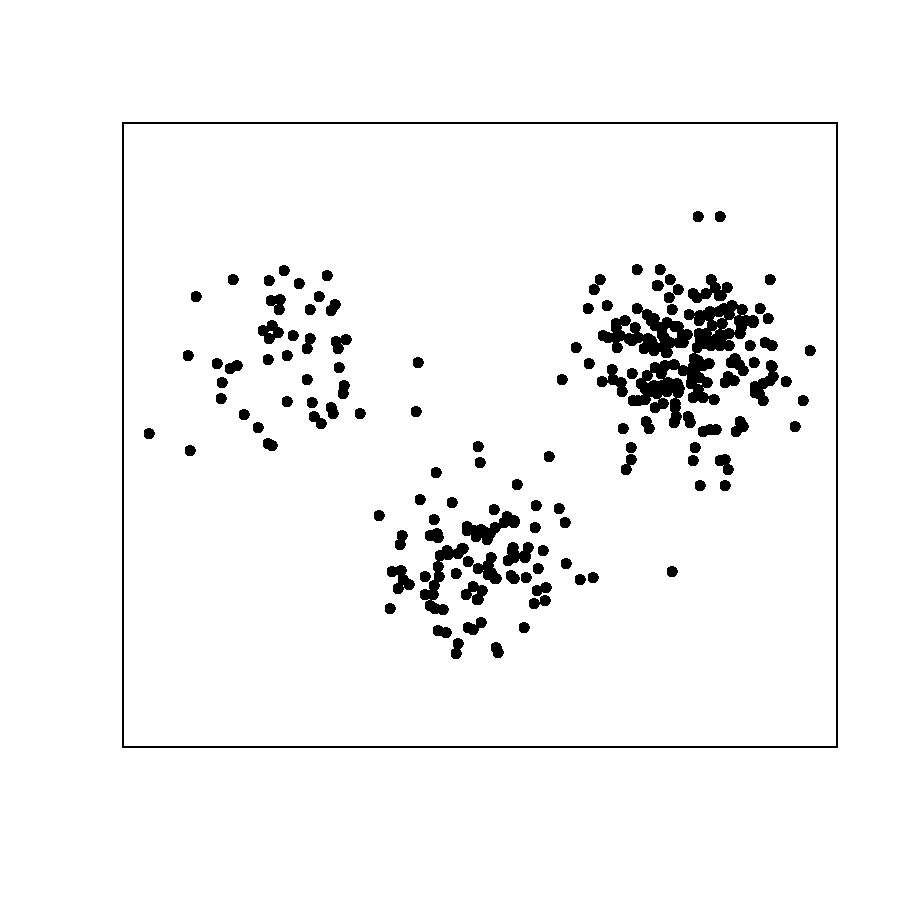
\includegraphics[scale=0.6]{kmeans-1}\hspace*{-1.7cm}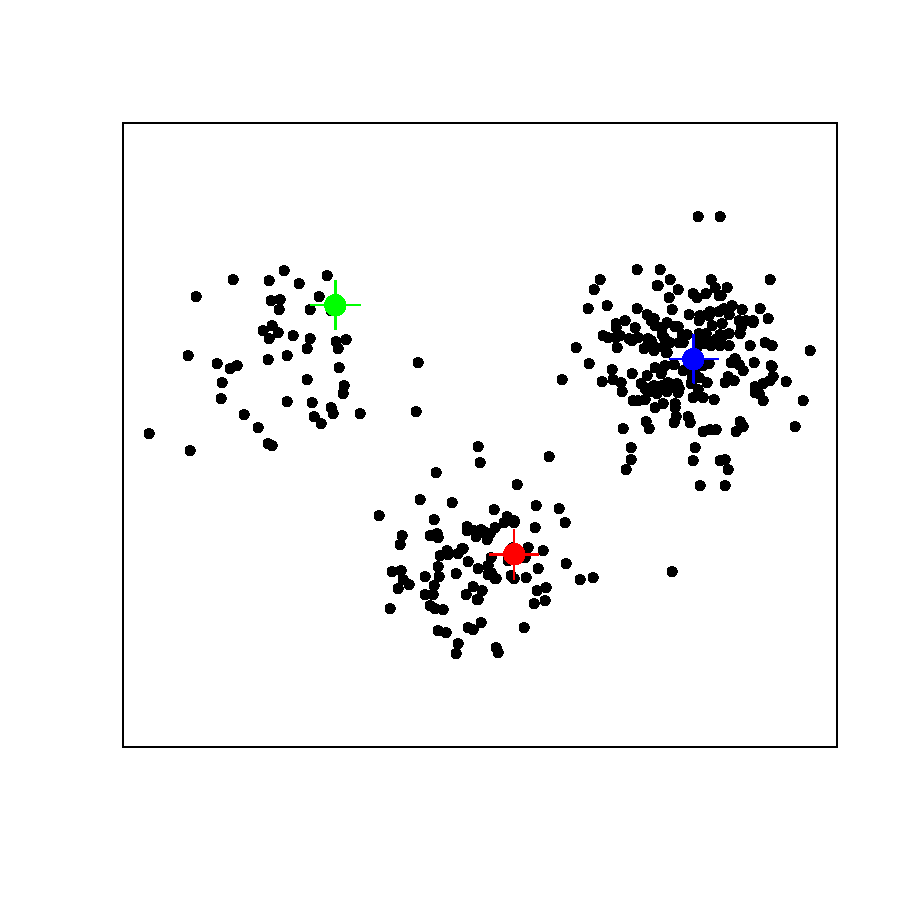
\includegraphics[scale=0.6]{kmeans-2}
\vspace*{-2.6cm}}

\centerline{
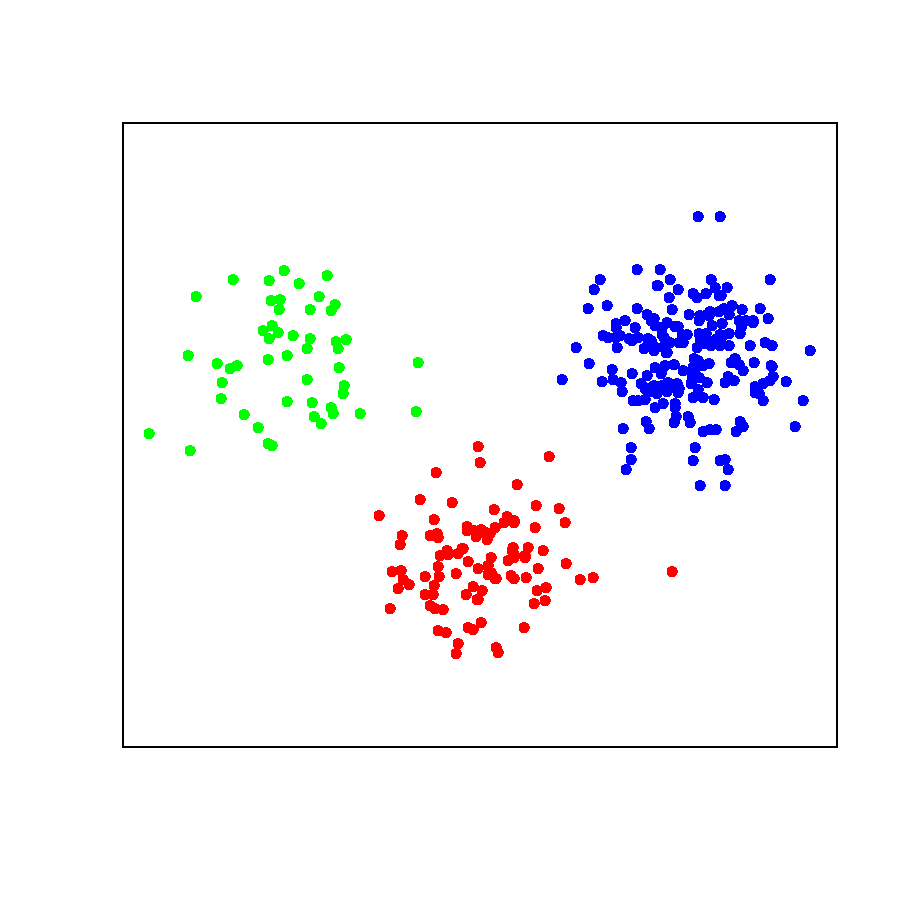
\includegraphics[scale=0.6]{kmeans-3}\hspace*{-1.7cm}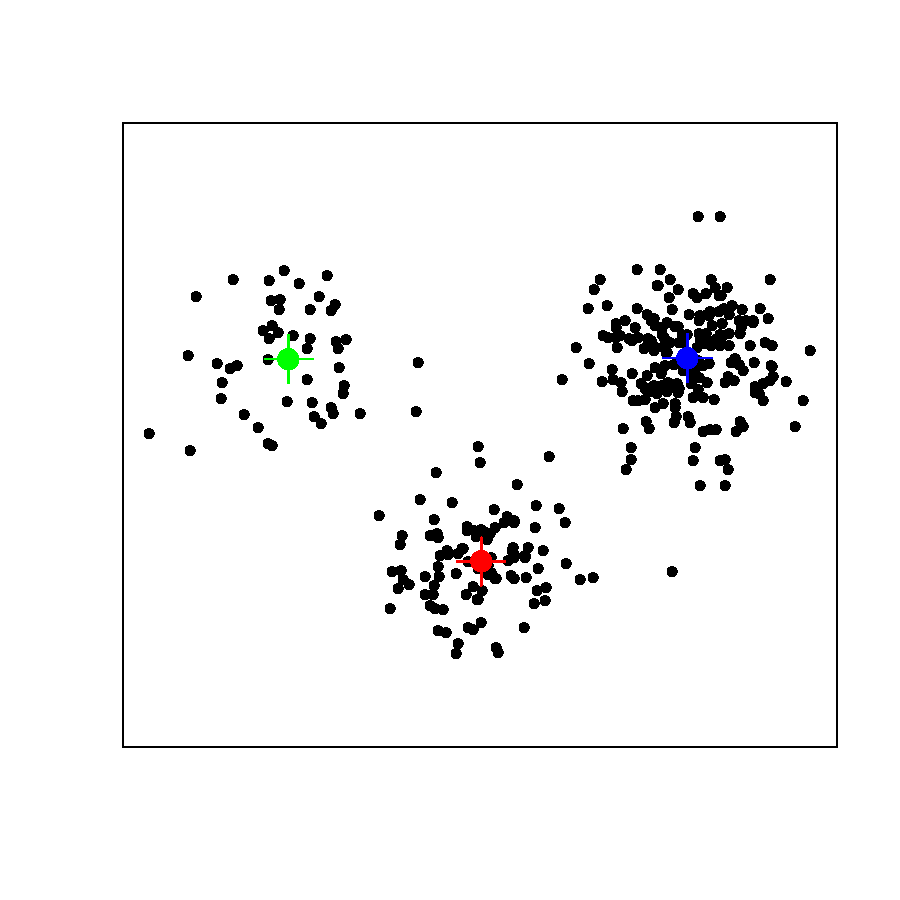
\includegraphics[scale=0.6]{kmeans-4}
\vspace*{-3.2cm}}

\foilhead[-1cm]{Example of suboptimal behaviour}

\centerline{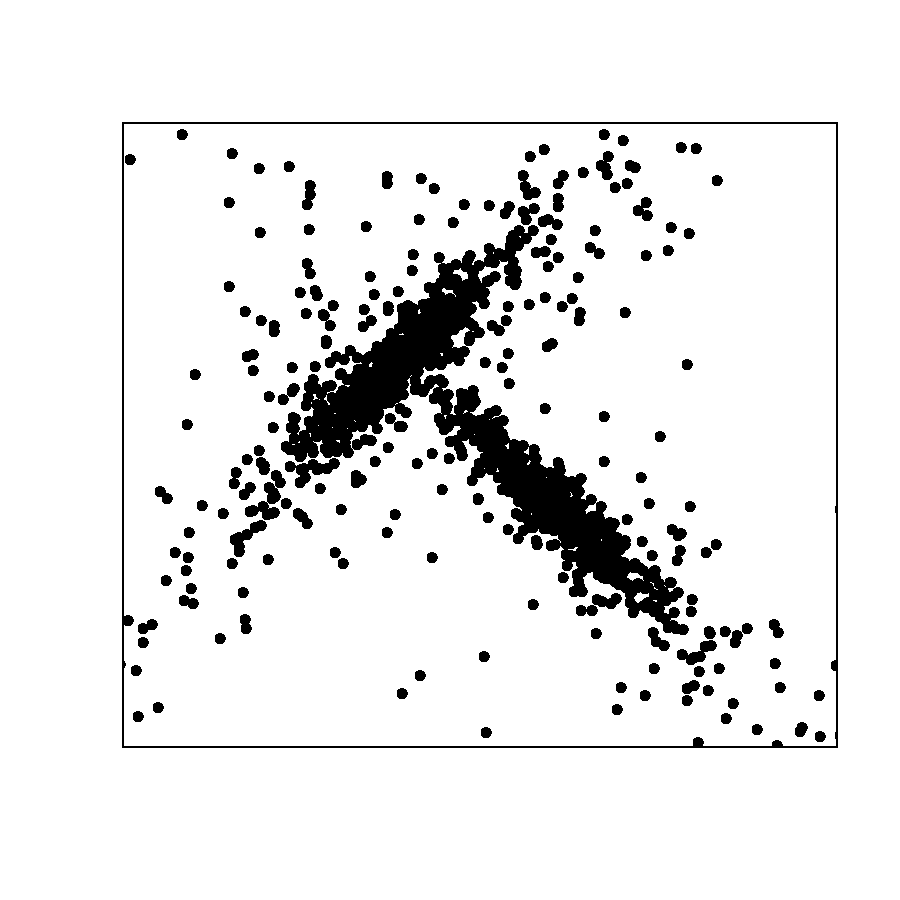
\includegraphics[scale=0.8]{kmeans-failure-1}\hspace*{-1.7cm}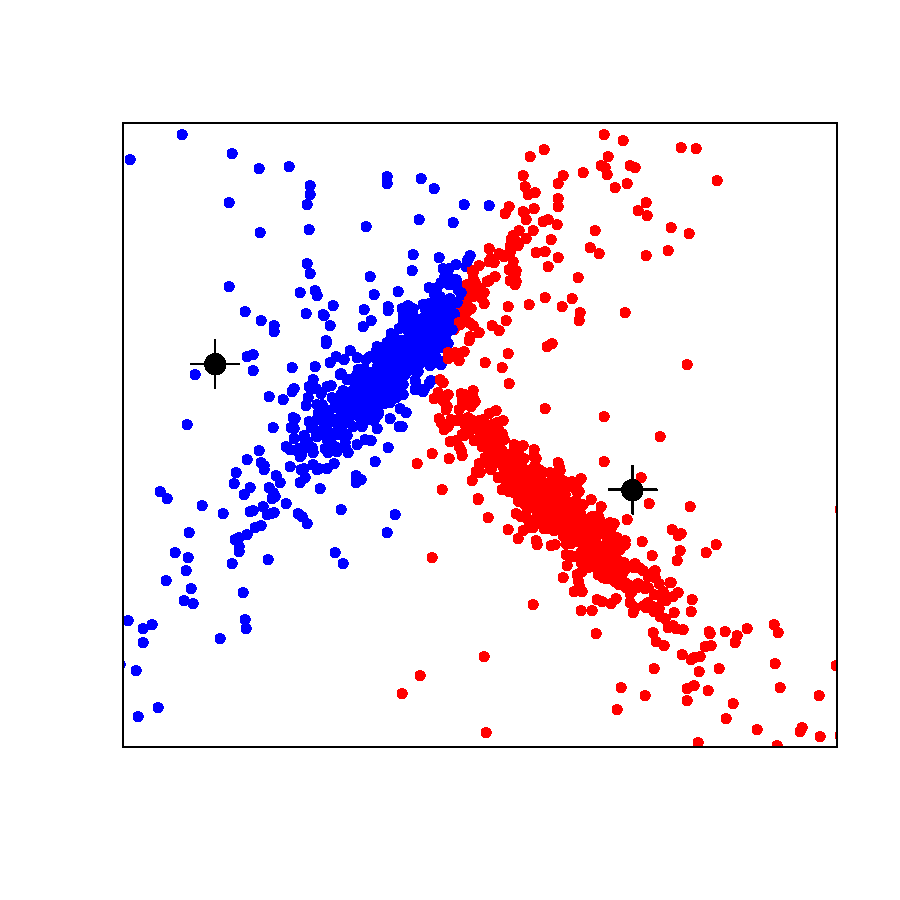
\includegraphics[scale=0.8]{kmeans-failure-2}}
\vspace*{-2cm}

K-means algorithm fails if clusters are elongated or one clusters have different density. In both cases the assumptions are not satisfied. 


\foilhead[-1cm]{Model for elongated clusters}

\begin{triangles}
\item Components of the underlying true noise  are samples as $\varepsilon_i\gets\NNN(0,1)$
\item Noise is reshaped using linear transformation $\vec{\varepsilon}_*=A\vec{\varepsilon}$
\item The final output is generated as $\vec{x}=\vec{\mu}+\vec{\varepsilon}_*$ 
\end{triangles}
\vspace*{1cm}


\textbf{Correponding mathematical model.} It is straightforward to express the corresponding probability density function
\begin{align*}
\pd{\vec{x}|\vec{\mu},A}&=\frac{1}{(\det A^TA)^{1/2}}\cdot\prod_{t=1}^d\frac{1}{\sqrt{2\pi}}\cdot\exp{-\frac{\varepsilon_t^2}{2}}\\
\pd{\vec{x}|\vec{\mu},A}&=\frac{1}{(2\pi)^{d/2}(\det AA^T)^{1/2}}\cdot\exp{-\frac{1}{2}\cdot (\vec{x}-\vec{\mu})A^{-T}A^{-1}(\vec{x}-\vec{\mu})}
\end{align*} 
where $\Sigma=AA^T$ is known as correlation matrix


\foilhead[-1cm]{Maximum likelihood estimates}

Multivariate normal distribution (\emph{coloured Gaussian noise}) $\NNN(\vec{\mu}, \Sigma)$ is completely determines by the centre $\vec{\mu}$ and correlation matrix $\Sigma$. 

It is straightforward though tedious to verify that parameter values that maximise the likelihood of data $\vec{x}_1,\ldots,\vec{x}_n$ can be competed as follows
\begin{align*}
\vec{\mu}&=\frac{1}{n}\cdot\sum_{i=1}^n \vec{x}_i\\
\Sigma&=\frac{1}{n}\cdot X_c^T X_c
\end{align*}
where $X_c$ is a $n\times d$ matrix obtained by staking $(\vec{x}_1-\vec{\mu})^T,\ldots,(\vec{x}_n-\vec{\mu})^T$.

\foilhead[-1cm]{Gaussian mixture model}

\begin{triangles}
\item There are $k$ different data sources $\DDD_1,\ldots,\DDD_k$
\item Each data source has a fixed centre $\vec{\mu}_j\in\RR^d$ and covariance matrix $\Sigma_j$
\item To sample data from  $\DDD_j$, we output $\vec{x}=\vec{\mu}_j+\vec{\varepsilon}$ for $\varepsilon\gets\NNN(\vec{0},\Sigma_j)$ 
\end{triangles}

\vspace*{1cm}


\textbf{Correponding hard-clustering task.} Find model parameters $\vec{\Theta}$ and labels $\vec{z}$ such that the likelihood of the data is maximal:
\begin{align*}
\pr{\vec{x}_1,\ldots,\vec{x}_n|\vec{z},\vec{\Theta}}\to \max
\end{align*}


\foilhead[-1cm]{Two-step minimisation algorithm}

\textbf{Observations} 
\begin{triangles}
\item If parameters $\vec{\Theta}$ are fixed it straightforward to find best label for each data point. We must choose $z_i$ such that $\pd{\vec{x}_i|\vec{\mu}_i,\Sigma_i}\to \max$.
\item If labels are fixed then we can individually adjust the parameters $\vec{\mu}_j$ and $\Sigma_j$ for clusters. Mixture fractions can be recomputed as $\lambda_j=\abs{\III_j}/n$.
\end{triangles}

\vspace*{0.5cm}


\textbf{Corresponding hard-clustering algorithm}
\begin{triangles}
\item[1.] Choose a good initial values for cluster parameters
\item[2.] For each data point $\vec{x}_i$ find the best cluster $j$ and set $z_i=j$
\item[3.] Recompute cluster parameters over data points belonging to it
\item[4.] Repeat from the step 2 until nothing changes
\item[5.] Repeat with different starting points and report the best result   
\end{triangles}
\vspace*{-0.5cm}


\foilhead[-2.0cm]{The algorithm really works}

\centerline{
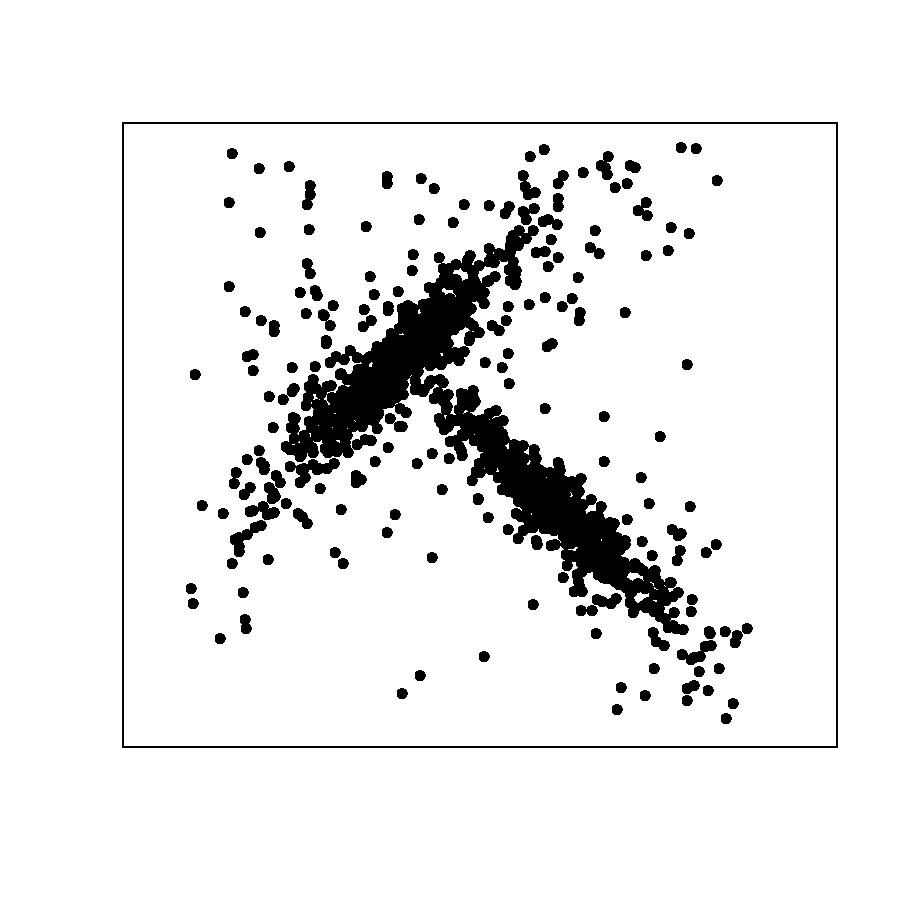
\includegraphics[scale=0.6]{hard-gmm-1}\hspace*{-1.7cm}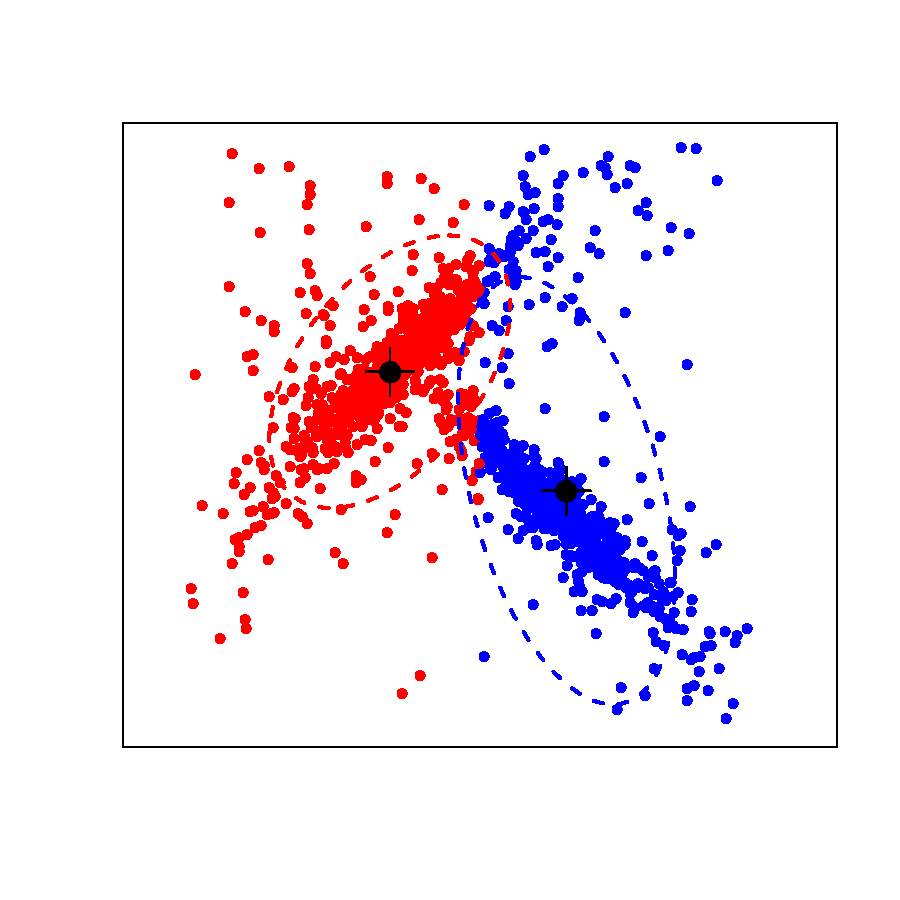
\includegraphics[scale=0.6]{hard-gmm-2}
\vspace*{-2.6cm}}

\centerline{
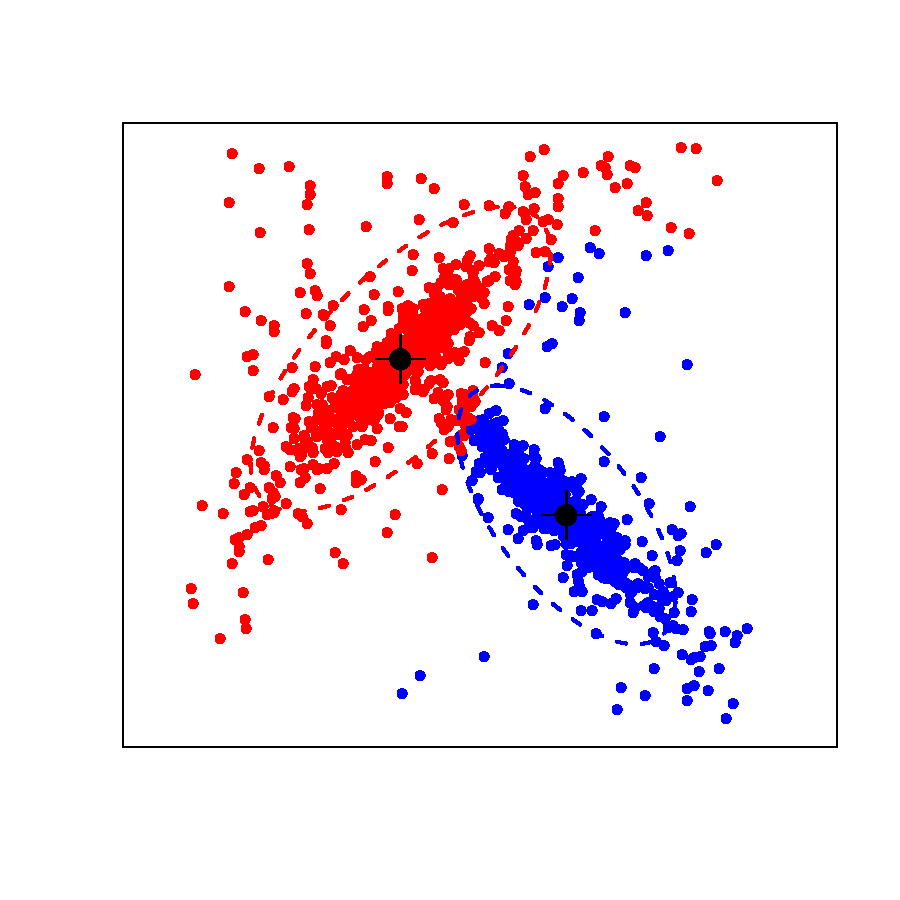
\includegraphics[scale=0.6]{hard-gmm-3}\hspace*{-1.7cm}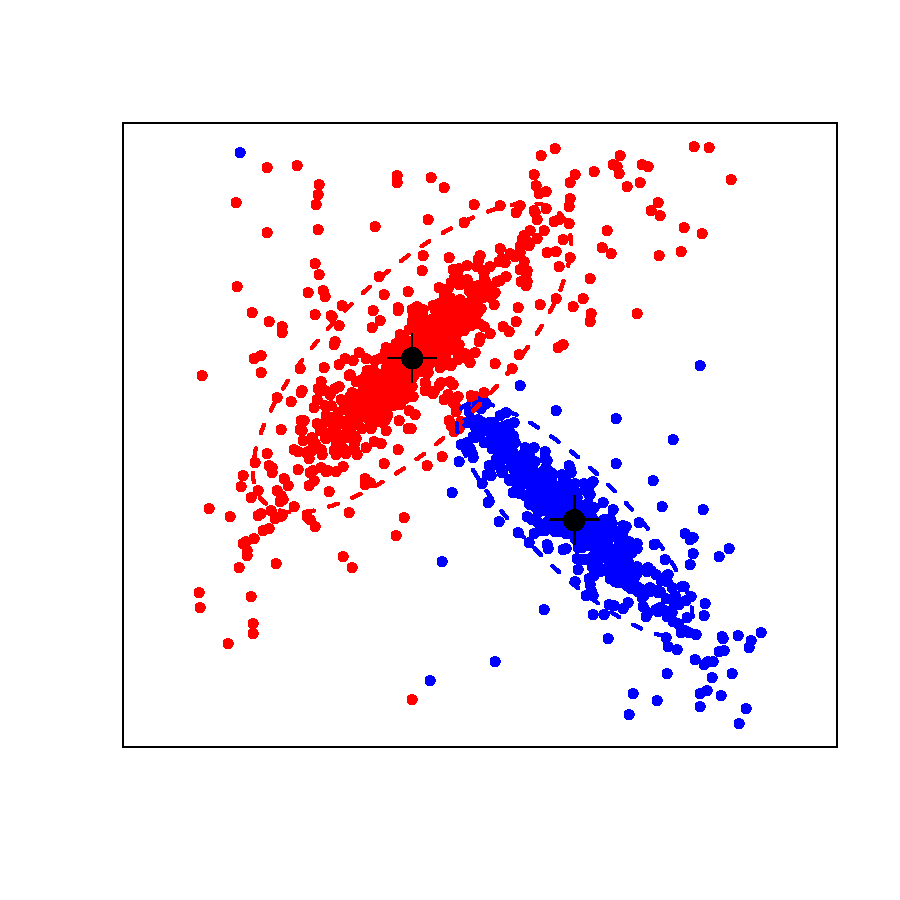
\includegraphics[scale=0.6]{hard-gmm-4}
\vspace*{-3.2cm}}

\foilhead[-1cm]{Hard datasets for the algorithm}

\centerline{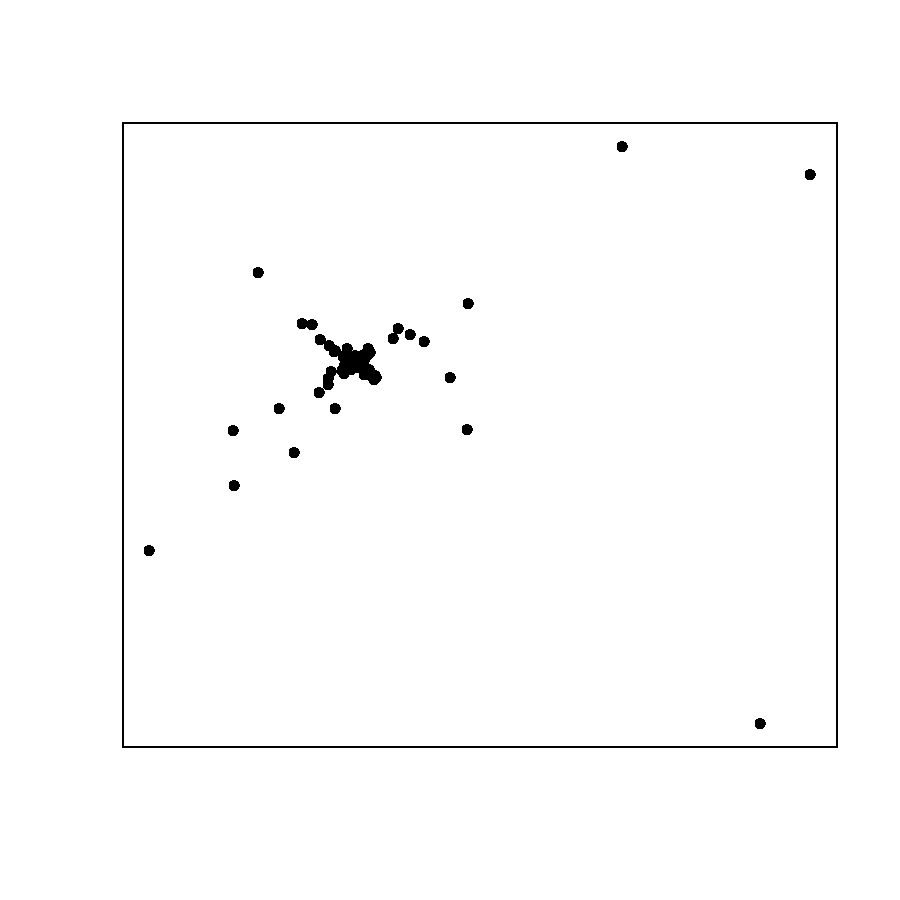
\includegraphics[scale=0.8]{hard-gmm-failure-1}\hspace*{-1.7cm}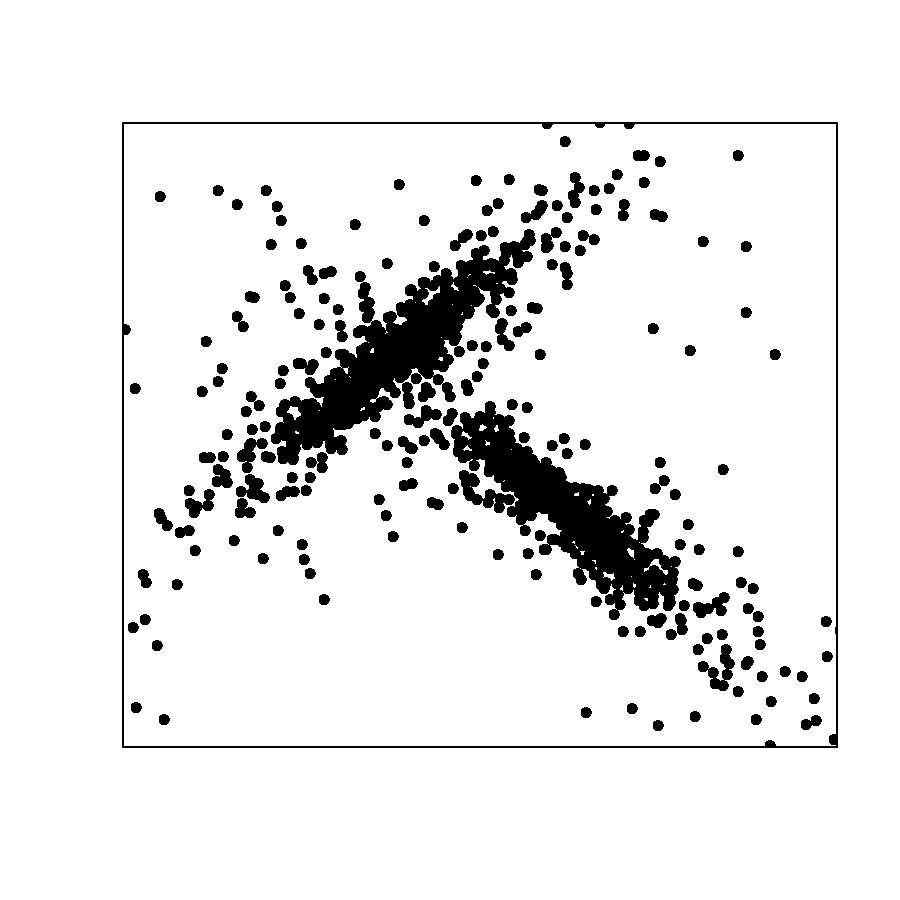
\includegraphics[scale=0.8]{hard-gmm-failure-2}}
\vspace*{-1cm}

Few extreme values can completely offset the hard-clustering algorithm. The latter is the weakness of the Gaussian mixture model.\vspace*{-0.5cm}


\end{document}
